\newpage
\section{Design and Implementation}
This section is dedicated to explaining the language and library used in implementation, an extension of the library method, and the implementation of the chosen encoding schemes and three key storage used in the encoding.

    \subsection{Programming Language}
I used \textbf{Python} for the implementation. Although python programs are generally expected to run slower than some other Object-oriented programming languages like JAVA and C++, it enables the programs to become three to five times shorter than JAVA and five to ten times shorter than C++.\footnote{https://www.python.org/doc/essays/comparisons/}, 
and Python also supports powerful dictionary and list types. \\

\noindent Another reason for using Python is that with certain libraries, Bayesian Networks can be imported or defined in a simple way, so that it supports testing the performance with widely used benchmarks.

\subsection{Input format}
The input is the \textbf{Bayesian Interchange Format} (BIF) which are files with .bif extension to represent Bayesian Networks. The BIF files are used as input because it's a widely used format in tools that are dealing with Bayesian Networks including BayesiaLab \footnote{http://www.bayesia.com/}, JavaBayes\footnote{https://www.cs.cmu.edu/~javabayes/Home/} etc, so there are a lot of available benchmarks with the BIF Format. In general, Four types of blocks are defined.\\

\noindent \textbf{The Network Block:}\\
\noindent A network block defines the name of the network and lists the properties. The example below specify the network block for the Asia Bayesian Network:
\begin{lstlisting}
network asia{
  property version 1.1;
  property author ..;
}
\end{lstlisting}

\noindent \textbf{The Variable Block:}\\
Variable blocks define the variables in a network. These blocks used
to be called node blocks in the BIF; it seems that variable conveys
more of a statistical meaning while node just refers to a graphical
concept. The example below is the bronc node from asia.bif
\begin{lstlisting}
 variable bronc{
    type discrete [2] {yes, no};
 }
\end{lstlisting}

\noindent \textbf{Blocks for standard nodes}\\
Standard nodes have to define the probabilities for each discrete parent instantiation. An example of a standard probability block is: 
\begin{lstlisting}
 probability (dysp | bronc, either){
    (yes, yes) 0.9, 0.1;
    (no, yes) 0.7, 0.3;
    (yes, no) 0.8, 0.2;
    (no, no) 0.1, 0.9;
}
\end{lstlisting}

\noindent \textbf{Probability blocks}:\\
Probability blocks are another way to specify the (conditional) probability tables (CPTs). For these variables, and hence the topology of the network. The block indicates the variables of the probability distribution right after the keyword probability.
\begin{lstlisting}
probability (v_10_8 v_10_7 v_9_8){ 
table 0.586357 0.667473 0.789088 0.466932 
      0.413643 0.332527 0.210912 0.533068;
}
\end{lstlisting}
A more detailed explanation of the BIF is explained here: \footnote{http://www.cs.washington.edu/dm/vfml/appendixes/bif.htm} \\

\subsection{Output}
The output of the program is the cnf file following the DIMACS format which is a widely accepted standard format for representing CNF clauses and it's also the input format used by most of the model counters mentioned in section 3.3.\\
\begin{itemize}
    \item A comment line starts with a \textit{c}
    \item A line p cnf var clauses specify the instance in CNF format, in which \textit{vars} is the number of variables used in the file and \textit{clauses} is the number of clauses in the CNF.
    \item Each CNF variable is denoted by a non\-zero number smaller than \textit{vars}, the negation of a variable is denoted by a negative number.
    \item Each clauses contains one or several CNF variables, 0 specifies the end of the clause.
\end{itemize}

Consider the following CNF:
\begin{center}
    $x_{1} \vee x_{2} \vee \neg x_{3}$\\
    $x_{1} \vee x_{4} \vee x_{5}$\\
    $\neg x_{3} \vee \neg x_{4}$\\  
\end{center}
The clauses in DIMACS format:
\begin{center}
    \begin{lstlisting}
    c A sample DIMAC file
    p cnf 5 3
    1 2 -3 0
    1 4 5 0
    -3 -4 0
    \end{lstlisting}
\end{center}
    
\subsection{Pgmpy}
The library to read and represent Bayesian networks is Pgmpy \cite{pgmpy_paper}. With Pgmpy, Bayesian network can be easily created, and it also support reading Bayesian networks from BIF format. The library is opensource so that it can be modified and extended if required. Pgmpy also have build-in inferencing method using Variable Elimination so that the run time can be used to evaluate the performance. 

 \subsection{Extend the Pgmpy library}
    Pgmpy library does not support fetching CPT values using table indexing, the only way to fetch value is through specifying evidence and variables and query the value through Variable Elimination method. The Variable Elimination method is the bayesian inference method that is \textcolor{red}{Insert time complexety}. To solve the problem, I extended the pgmpy library to support fetching variable values without querying using Variable Elimination.\\

    \noindent \textbf{The TabularCPD Class}:\\
    The method get\_cpds returns a conditional probability distribution of the node, the returned type is defined as TabularCPD that contains the name of the node, cardinality, variables which are stores as a nested list, the list of evidences and their corresponding cardinalities. An example is given below:
    \begin{lstlisting}
    cpd = TabularCPD('dysp', 2, [[0.9, 0.7, 0.8, 0.1],
                                 [0.1, 0.3, 0.2, 0.9]],
                                 ['bronc', 'either'], [2, 2])
    \end{lstlisting}

    \noindent \textbf{The storage of a TabularCPD}:\\
    calling cpd.variables() will return a list starts with the node variable followed by the the evidences, and calling cpd.cardinality() will return the cardinality list in the same order as the variables returned by cpd.variables()
    \begin{lstlisting}
    >> print(cpd.variables())
        >> ['dysp', 'bronc', 'either']
    >> print(cpd.cardinality())
        >> ['2', '2', '2']
    \end{lstlisting}

   \noindent \textbf{MyCPD}:\\
    col\_index stores the index of the combination of evidence, in the same order as the probability distribution defined in the \textbf{standard node block}. The col\_index is constructed using the itertools.product in python which return the cartesian product. The transpose of the col\_index correspond to the order of the probability distribution specify in the BIF file. Consider the example with node \textit{dysp}.
    \begin{lstlisting}
    >> col_indexes = np.array(list(product(*[range(i) for i in ev_card])))
    >> print(evidence, col_index) 
        >> ['either', 'bronc']
        >> [[0 0]
            [0 1]
            [1 0]
            [1 1]]
    \end{lstlisting}
   
    \noindent Then the evidences are formatted into tuples with the same length and each column correspond to one entrance to the probability table.\\
    \begin{lstlisting}
    A sample return the evidence entrance. 'dysp' node in aisa.bif
    >> entrance <- [('{s}'.format(s = reverse_ev[i]), d) 
                    for d in col_indexes.T[i]]
        >> [('either',0), ('either',0), ('either',1), ('either',1)]
           [('bronc', 0), ('bronc', 1), ('bronc', 0), ('bronc', 1)]
    Then the entrace are transposed using rol_to_col()
    >> rol_to_col(entrance)
        >> [[('bronc',0), ('either',0)], [('bronc',1), ('either',0)], 
            [('bronc',0), ('either',1)], [('bronc',1), ('either',1)]]
    \end{lstlisting}
    
    \begin{minted}
    [linenos]
    {python}
    Parameter: A TabularCPD
    def myCPD(TabularCPD cpd):
        var, evidence <- cpd.variable[0], cpd.variable[1:]
        var_card, ev_card <- cpd.cardinality[0], cpd.cardinality[1:]
        variable <- [(name, 0),.., (name, n)]
        value = cpd.values()
        # node with evidence:
        if evidence not null:
            col_indexes <- get index
            for i in cardinality:
                entrance <- format the header
                rol_to_col(entrance) # transpose
            for each node variable:
                newcpt.append(variable, index, evidence, corresponding_value)
        # node with no evidence
        else:
            for each node variable
                newcpt.apend(variable, index, [], corresponding_value)
    \end{minted}
    A Sample return of newcpt of node dysp:
    \begin{lstlisting}
    [('dysp', 0, [('bronc', 0), ('either', 0)], 0.9), 
     ('dysp', 0, [('bronc', 1), ('either', 0)], 0.7), 
     ...
     ('dysp', 1, [('bronc', 0), ('either', 1)], 0.2), 
     ('dysp', 1, [('bronc', 1), ('either', 1)], 0.9)]
    \end{lstlisting}
    The method mycpd(TabularCPD) returns a table\-like list of tuples, the first two element in each tuple forms the node variables and the third element is a list of evidence. An example of the first tuple in the list means $dysp_{0}|bronc_{0}either_{0} = 0.9$. Now the returned data support fetching values using list indexing so that we don't need to query the value using the time-consuming Variable Elimination.\\ 
    
    
    \noindent In our case for both bronc and either, the evidence all equals to 2, the convention for the order is shown in figure \ref{fig:sample print table}. The list which store the values are the transpose of the matrix in BIF format.\\
    \begin{figure}
        \centering
        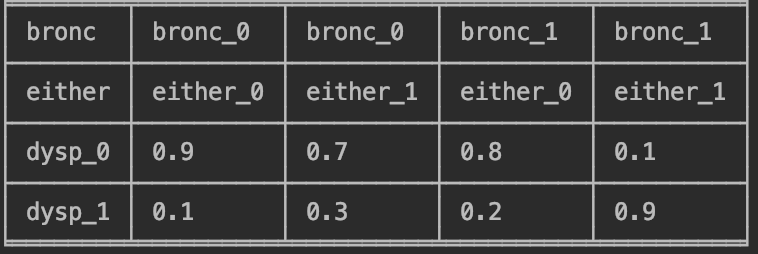
\includegraphics[width = 0.7\textwidth]{pic/printBayesnode.png}
        \caption{A sample printed CPT of a node dyps}
        \label{fig:sample print table}
    \end{figure}
    
\subsection{Storing variables, weights and CNFs}
There are three important storage in the implementation, the generated variables, corresponding weights and the representation of CNFs.\\

\noindent Variables in the CNFs and its corresponding weights are stored in python dictionaries. One of the consideration is the speed of looking up  a certain variable weights or its corresponding integer used in the DIMAC format. Encoding Bayesian networks might lead to dealing with large number of variables. Some of the results \cite{2008-literature-review} shows that the variable numbers might reach over 50,000. \\

\noindent If we use a list of pairs to store the variables or the weights, the time complexity for looking up a list is \textbf{O}(n) for linear search over the list. However, the time complexity for looking up in the dictionary is \textbf{O}(1). When dealing with large number of variables, the time difference is substantial. In addition, adding the dictionary operation 'add' is an process with O(1) regardless of the size of the dictionary. The key in the variable is the name of the variable, \textit{weights} stores its corresponding weight and the var\_dic stores the integer used to represent the variable in the DIMAC format.

\begin{lstlisting}
var_dic = {
    'theta_x1|y1y2': 5,
    ...
}

weights = {
    'theta_x1|y1y2': 0.03,
    ...
}
\end{lstlisting}

\noindent The CNF clauses are stored as a list of lists. Inner list represent one clause that are the disjunction of literals, and the outer list represent the conjunction of the clauses. We use list to store the clauses because once a clause is generated and append to the list, it won't be modified during the later process, and no other operation such as list lookup is needed. The only operation is to traverse each clause in the list that the CNF to write to files.

    \subsection{Implementation of Full encoding}
    In section 3.1 Full encoding, for each node in the Bayesian network, two kinds of variables need to be generated, indicator variables and parameter variables respectively. This section will first show the steps to generate indicator variables and indicator clauses and then show the steps to encode parameter variables and clauses.
    \begin{itemize}
        \item \textit{var\_dic} is a dictionary in which the key is the name of the variable and the value is used when the cnf is written into the DIMACS format. 
        \item \textit{clauses} is a nested list, each element correspond to one clauses in the generated CNF. Literals are stores as a tuple (sign, variable). sign = -1 means the negation of the variable
        \item \textit{weights} is a dictionary that stores the corresponding weights of the variable following the weights assigning rules mentioned in section 3.2.2. The key is the name of the variable such as $\lambda_{dysp_{0}}$ and the value is the corresponding weight.
    \end{itemize}
    \textbf{Generating Indicator variables:}\\
    Given a bayesian network \textit{bn}, for each node in the network, define the number of indicators same as its cardinality. Then two types of clauses are generated: $[\lambda_{x_{1}}, ... \lambda_{x_{n}}]$ and $[\neg \lambda_{x_{i}}, \neg \lambda_{x_{j}}]$ when $i < j$. weights($\lambda_{x}$) = 1, weights($\neg \lambda_{x}$) = -1. Traverse the node in the given Bayesian network and all indicator clauses are generated.
    The Psuedocode for generating indicator variables and clauses is given below:
    \begin{minted}
    [linenos]
    {python}
    def indicator(bn, var_dic, clauses, weights):
        for i in bn.nodes:
            cardinality <- bn.get_cardinality(i)
            # get variables
            for j in range(cardinality):
                name <- 'lambda_' + str(i)+ '_' + str(j)
                # append variable to variable dictionary
                # store the corresponding weights
                if name not in var_dic:
                    var_dic[name] = max(var_dic.values()) + 1
                    weights[name] = 1
            # get clauses:
        for i in bn.nodes:
            cardinality <- bn.get_cardinality(i)
            cl = [] # cl store each clause in the CNF, represented by a list of tuples
            for j in range(cardinality):
                variable <- fetch the corresponding variable from the dictionary
                cl.append((1, variable)) # 1 represent positive
            clauses.append(cl)
            
            for m in range(cardinality):
                for n in range(m + 1, cardinality):
                    var1, var2 <- fetch lambda_i_n, fetch lambda_i_m
                    cl = [(-1, var1), (-1, var, var2)]
                    clauses.append(cl)
                    weights[m] = -1
    return clauses, var_dic, weights
    \end{minted}
    
    \noindent \textbf{Generating Parameter variables:}\\
    For each variable of a node in the bayesian network, first get the evidence of the variable and the the evidences' cardinality. These, together with the node's cardinality, specify the number of values in a conditional probability table. For each value, a parameter variable $\theta_{node_{i}|evidences}$ is generated.\\
    $$number\_of\_values = cardinality(node) \times \Pi_{i = 1}^n cardinality(evidence_{i})$$
    
    The corresponding clauses: (described in line 20 \~ 26 in psuedocode)
    \begin{itemize}
        \item $ \neg\lambda_{x_{i}} \vee \neg\lambda_{y_{1}} \vee... \vee \neg\lambda_{y_{m}} \vee \theta_{x_{i}|y_{1}..y_{m}}$
        \item  $\neg\theta_{x_{i}|y_{1}..y_{m}} \vee \lambda_{x_{i}}$
        \item $\neg\theta_{x_{i}|y_{1}..y_{m}} \vee \lambda_{y_{j}} \;\; \mbox{ j = 1, ..., m}$
    \end{itemize}
    
    \begin{minted}
    [linenos]
    {python}
    def parameter_cl(bn, var_dic, clauses, weights):
        for i in bn.nodes:
            cardinality = i.get_cardinality()
            evidence = i.get_evidence()
            if no evidence:
                for j in cardinality:
                    name <- theta_ij
                    var_dic[name] <- max(var_dic.value()) + 1
                    weight[name] <- fetch weight
                    clauses.append([(-1, var_dic['lambda_i']), (1, var_dic[name]])
                    clauses.append([(-1, var_dic[name]), (1, dic['lambda_i'])])
            else:
                ev_cardinality <- [ev.cardinality() for ev in i.evidence]
                evidence_lst <- generate evidence list()
                for j in cardinality:
                    for ev in evidence_lst:
                        name = 'theta_' + i + str(j) + '|' + ev
                        var_dic[name] <- max(var_dic.value()) + 1
                        weight[name] <- fetch weight
                        clauses.append([(-1, var_dic['lambda_i']),
                                        ...
                                        (-1, var_dic['lambda_evidences']),
                                        (1, var_dic[name]])
                    clauses.append([(-1, var_dic[name]), (1, dic['lambda_i'])])
                    ...
                    clauses.append([(-1, var_dic[name]), (1, dic['lambda_evs])])
        return var_dic, clauses, weights
    \end{minted}
    % \caption{Psuedocode for encoding parameter clauses}
    % \label{code:Full enc parameter clauses}

    \subsection{Simplified Full encoding}
    In simplified Full encoding, one of the main improvement is to capture the extreme values when generating the parameter clauses. Before generating variables and clauses, the weight is fetched from the Probabilty table.\\
    \newline
    \noindent If Pr($variable_{i}|evidence_{1}...evidence-{m}$) = 0, the parameter clauses won't be generated, and only one clause will be appended to the CNF: [$\neg \lambda_{variable_{i}|}, \neg \lambda_{evidence_{1}}, ..., \neg \lambda_{evidence_{m}}$].\\
    
    \noindent If Pr($variable_{i}|evidence_{1}...evidence-{m}$) = 1, no action is done and the program should move to the next entry of the probability table.\\
    
    \noindent The psuedocode for simplifying extreme values with evidence list not empty is given below, the case without evidence can be implemented similarly.
    \begin{minted}
    [linenos]
    {python}
    for i in bn.nodes:
        for j in i.get_cardinality():
            evidence = i.get_evidence()
            # case with evidence:
            if evidence not null:
                parameter_value <- fetched weight
                if parameter_value == 0:
                    clauses.append([(-1, var_dic[lambda_ij]),
                                    (-1, var_dic[lambda_evidence1]), 
                                    ... ,
                                    (-1, var_dic[evidence_m])])
                if parameter_value == 1:
                    continue
                else: 
                    do the same as Full encode parameter clauses
        
    \end{minted}
    According to \cite{enc1}, the simplification step lead to significant improvement in the number of clauses which directly influence the time and space usage in the model counting phase. Detailed result is discussed later in the Result section.
    
    \subsection{Implementation of Improved Encoding}
    The idea of Improved encoding is to use same logic variable to encode the parameter variables that have the same value in the CPT. For each node in the Bayesian network, the table is first partitioned in to several sub-tables based on the non-extreme probability values. This can be done with the sorting within the table fetched by myCPD(TabularCPD) method. After the partition of the table, an encoding scheme for paramter values and clauses is described.
    
    \subsubsection{Encoding each parameter value}
    If the value is unique or extreme (0 or 1), it's considered a subgroup itself. For each subgroup, let \textit{p} denotes each row in the subgroup, the following algorithm describes the encoding step for each subgroup.
    \begin{algorithm}
    \caption{Improved Encoding for each subgroup}\label{algorithm:encode group}
    \begin{algorithmic}[1]
    \Procedure{$Subgroup\_encode$}{$sub\_group$, $clauses$}
    \For{$each sub-group \tau $}
    \State $P \gets$ each row \textit{p} in subgroup \Comment{Assume $x_{1}, ev_{1}, ..., ev_{m}$ in p}
        \State \textbf{I} $\gets$ lambda\_xi, lambda\_ev1, .. lambda\_evm
            \Comment{I $\gets$ encodes p}
        \For{each p}
            \If {$\theta = 0$}
                \State continue
            \EndIf
            \If {$\theta = 1$}
                \State $clause \gets \neg I$
                \State clauses.append(clause)
            \Else
                \State $clause \gets \neg I \vee \theta_{index}$
                \State clauses.append(clause)
            \EndIf
        \EndFor
    \EndFor
    \State \textbf{return} $clauses$
    \EndProcedure
    \end{algorithmic}
    \end{algorithm}
    \subsection{Implementation of Group Encoding}
    \subsubsection{QM algorithm}
    QM algorithm, proposed by Quine and McClusckey, is an algorithmic way of simplifying Boolean logic functions. The library for QM algorithm applied for binary variables were used and extended to support the simplification for multi-variables.
    
    \subsubsection{An extension of QM algorithm for multi-variate simplification}
    To simplify multi\-variate Bayesian network variables, the QM algorithm were extended.\\
    
    \noindent For the variables in the CPT, a fixed length of bit string is used to represent the combination of variable. The length of bit string depends on the cardinality of each variable. 
    $$total\_length = \Sigma_{i = 1}^{m} \lceil log_{2}(Cardinality(Var_{i}))\rceil$$
    The bit string is then transformed from binary to decimal numbers as the input of QM algorithm. Then the output is spitted into small binary groups same as the length used to encode each variable. 'X' means the don't care case. If given values of for the other variables, the variable contains the don't care case will have a uniform probability or irrelevant, variable can be removed from the clause. Table \ref{tab:QM encode} gives and example for the extension. \\
    
    \begin{table}[]
        \centering
        \begin{tabular}{c c c c |c c}
            \hline
            Dysp & Bronc & Either & Pr & bitstring & decimal \\
            \hline
            \hline
             1 & 1 & 1 & 0.9 & 111 & 7 \\
             1 & 0 & 1 & 0.9 & 101 & 5 \\
             0 & 0 & 0 & 0.9 & 000 & 0 \\
            \hline
            card = 2 & card = 2 & card = 2 & -- & -- & -- \\
            \hline
        \end{tabular}
        \caption{An example of encoding using dysp node in asia.bif}
        \label{tab:QM encode}
    \end{table}
    
    \noindent This extension of the QM algorithm won't simplify the clauses into the most essential prime implicants for variables with cardinality $\>$ 2, while it the simplification of the encoding result already lead to significant improvement into number of clauses.\\
    
    \noindent Smaller clauses may be generated if we apply the algorithm multiple times while the runtime of QM algorithm is exponential to the size of variables. Therefore, the algorithm is only applied once for each subgroup of the CPD.\\
    
    \begin{lstlisting}
    An example process using the table mentioned above
    >> bitstring(table)
    >> qm.qm(ones = [0, 5, 7])
        >> ['000', '1X1']
    >> split_result(['000', '1X1'])
        >> [['0', '0', '0'], ['1', 'X', '1']]
    >> decode_qm_output -> [[Dyspnea_0, Bron_0, Either_0],
                            [Dyspnea_1, Either_1)]]
    \end{lstlisting}
    
    \noindent The output of the extendedQM(subgroup) is the simplified implicants of the subgroup. For each output, the following encoding steps are used to generated clauses:
    
    \begin{algorithm}
    \caption{Group Encoding for each subgroup}\label{algorithm:group encoding}
    \begin{algorithmic}[1]
    \Procedure{$Subgroup\_encode$}{$sub\_group$, $clauses$}
    \For{each sub-group $\tau$}
        \State P $gets$ output simplified groups from the extendedQM
        \State  I $gets$ lambda\_x1 , ... ,lambda\_evidence
        \For{each p}
            \If {$\theta = 0$}
                \State continue
            \EndIf
            \If {$\theta = 1$}
                \State $clause \gets \neg I$
                \State clauses.append(clause)
            \Else
                \State $clause \gets \neg I \vee \theta_{index}$
                \State clauses.append(clause)
            \EndIf
        \EndFor
    \EndFor
    \State \textbf{return} $clauses$
    \EndProcedure
    \end{algorithmic}
    \end{algorithm}

  
